%%%%%%%%%%%%%%%%%%%%%%%%%%%%%%%%%%%%%%%%%%%%%%%%%%%%%%%%%%%%%%%%%%%%%%%%
\section{Wiederholung}\label{K:wdh}
\begin{frame}
  \frametitle{\kap. Wiederholung}%
\tableofcontents[current]
\end{frame}


%%%%%%%%%%%%%%%%%%%%%%%%%%%%%%%%%%%%%%%%%%%%%%%%%%%%%%%%%%%%%%%%%%%%%%%%
\def\sstitle{Logische Operatoren}
\subsection{\sstitle}\label{S:LogiOperatoren}
\begin{frame}[fragile]%
  \frametitle{\kap.\ref{S:LogiOperatoren} \sstitle}%

Prüfe in welchem Quadranten ein Punkt mit den Koordinaten $x$ und $y$ liegt.

\begin{lstlisting}[style=java, frame=single]
// Punkt liegt im III Quadrant falls
if( x < 0 && y < 0 )
\end{lstlisting}
\begin{lstlisting}[style=java, frame=single]
// Punkt liegt in den Quadranten I, II, IV falls
if( x > 0 || y > 0 )
// equivalent zu 'nicht in III Quadrant'
if( !(x < 0 && y < 0) )
\end{lstlisting}
\end{frame}

%%%%%%%%%%%%%%%%%%%%%%%%%%%%%%%%%%%%%%%%%%%%%%%%%%%%%%%%%%%%%%%%%%%%%%%%
\def\stitle{De Morgansche Gesetze}
\subsection{\stitle}\label{S:Morgansche}
\begin{frame}[fragile]%
  \frametitle{\kap.\ref{S:Morgansche} \stitle}%
Vergleich Analysis I
\medskip

\begin{description}
  \item[und bzw. oder]
  \item $\neg \neg A = A$
  \item $\neg (A \wedge B) = \neg A \vee \neg B$
  \item $\neg (A \vee B) = \neg A \wedge \neg B$
\end{description}
\medskip

\begin{description}
  \item[Schnittmenge bzw. Vereinigung]
  \item $(A^{\mathsf{c}})^{\mathsf{c}} = A$
  \item $(A \cap B)^{\mathsf{c}} = A^{\mathsf{c}} \cup B^{\mathsf{c}}$
  \item $(A \cup B)^{\mathsf{c}} = A^{\mathsf{c}} \cap B^{\mathsf{c}}$
\end{description}
\end{frame}

%%%%%%%%%%%%%%%%%%%%%%%%%%%%%%%%%%%%%%%%%%%%%%%%%%%%%%%%%%%%%%%%%%%%%%%%
\def\sstitle{Priorität der Operatoren}
\subsection{\sstitle}\label{S:Prioritat}
\begin{frame}[fragile]
  \frametitle{\kap.\ref{S:Prioritat} \sstitle}%

\begin{lstlisting}[style=java, frame=single]
// Punkt for Strich
System.out.println(1+4/2); // Klammern 1+(4/2)
System.out.println(2+3%2); // Klammern 2+(3%2)
System.out.println(2*3%2); // Von links nach rechts
\end{lstlisting}
\hfill

Gegeben sei der folgende Java--Ausdruck:
\begin{center}
\code{a || b && c}
\end{center}
Dabei seien \code{a, b, c} Variablen vom Typ \code{boolean}.
\medskip

Wie wird dieser Ausdruck abgearbeitet (engl. \emph{operator precedence})?
\pause
\begin{enumerate}
  \item \code{ a || (b && c)}
\end{enumerate}
\pause
Welche der folgenden Ausdrücke ist die korrekte \textbf{Negation}?
\begin{enumerate}
  \item \code{!a && (!b || !c)}
  \item \code{!a &&  !b || !c}
\end{enumerate}

\end{frame}

%%%%%%%%%%%%%%%%%%%%%%%%%%%%%%%%%%%%%%%%%%%%%%%%%%%%%%%%%%%%%%%%%%%%%%%%
\def\stitle{Offizielle Dokumentation}
\subsection{\stitle}\label{S:Dokumentation}
\begin{frame}[fragile]%
  \frametitle{\kap.\ref{S:Dokumentation} \stitle}%
%%source
\textcolor{KITblue}{\url{docs.oracle.com/javase/tutorial/java/nutsandbolts/operators.html}}

\begin{center}
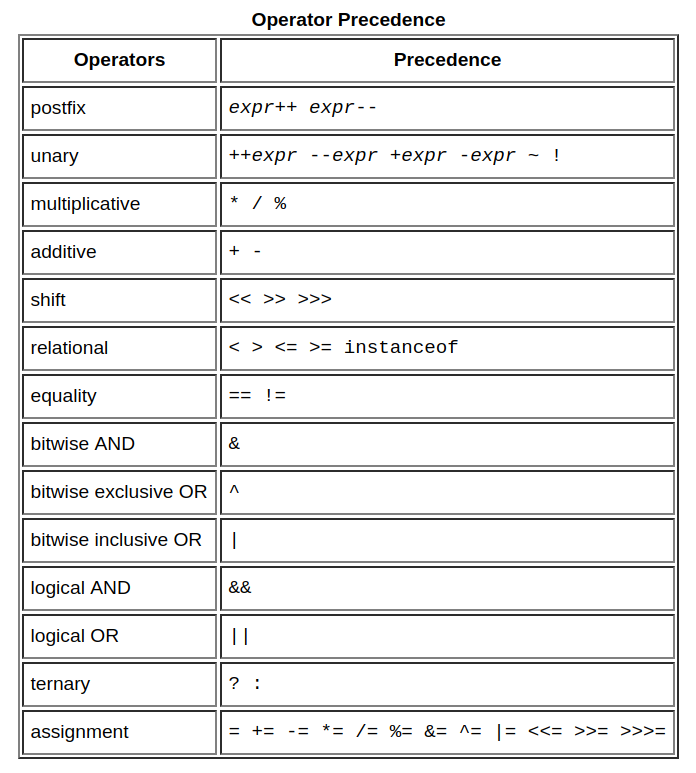
\includegraphics[width=0.5\textwidth]{\getexercisefolder/operatorPrecedence}
\end{center}
\end{frame}
